\chapter{Finite Elements}
{\color{blue} Ir viendo que algunas cosas de acá van a ir a parar
a Preliminaries.}
\section{Prismatic Finite Elements}
>this intends to be an extension of the treatment
in~\cite{giraultRaviart} to prismatic elements?
\subsection{Definici\'on del \emph{edge element} en prismas} % (fold)
\label{sub:defEdgeElement}
Now we introduce two polynomial spaces which will be used to construct 
the edge elements on the reference prism (Figure~\ref{reference_prism}).
\begin{defi} For an integer $k\geqslant 1$, let $R_k(\hat{T})$ denote the space of polynomials, defined over the
triangle $\hat{T}$, given by
\begin{IEEEeqnarray}{rCl}
    \label{defRk}
    R_k(\hat{T}) & := & P_{k-1}(\hat{T})^2 \oplus S_k(\hat{T})
\end{IEEEeqnarray}
where
\begin{IEEEeqnarray}{rClCrCl}
    \label{defSk}
    S_k(\hat{T}) & := & \{ \emph{\textbf{p}}\in \tilde{P}_k^2 \,:\;\emph{\textbf{p}}\cdot\emph{\textbf{x}} = 0\}$\quad$\emph{\textbf{x}} & = & (x_1, x_2).
\end{IEEEeqnarray}
\end{defi}
\noindent In order to establish unisolvence we need to calculate
$\dim\left(R_k(\hat{T}) \otimes P_k(\hat{I})\right)$.
\begin{IEEEeqnarray*}{rCl}
    \dim\left(R_k(\hat{T}) \otimes P_k(\hat{I})\right) 
    & = & \dim\left(R_k(\hat{T})\right) \dim\left(P_k(\hat{I})\right) \\
    & = & \dim\left(R_k(\hat{T})\right) (k+1).
\end{IEEEeqnarray*}
\begin{IEEEeqnarray*}{rCl}
    \dim\left(R_k(\hat{T})\right) 
    & = & \dim\left(P_{k-1}(\hat{T})^2 \oplus S_k(\hat{T}) \right)\\
    & = & 2\dim\left(P_{k-1}(\hat{T})\right) + \dim\left(S_k(\hat{T}) \right)\\
    & = & k(k+1) + \dim\left(S_k(\hat{T}) \right).
\end{IEEEeqnarray*}
Para la dimensi\'on de $S_k(\hat{T})$:
\begin{IEEEeqnarray*}{rCl}
S_k(\hat{T}) = \{ \textbf{p} \in \widetilde{P}_k^2 \, : \, \textbf{p}\cdot\textbf{x} = 0 \}.
\end{IEEEeqnarray*}
Consid\'erese
\begin{IEEEeqnarray*}{lll}
    \phi\,:\,\widetilde{P}_k^2 & \longrightarrow & \widetilde{P}_{k+1}\\
    \phi(\textbf{p})    & := & \textbf{p}\cdot\textbf{x}\\
                        & := & x_1p_1 + x_2p_2.
\end{IEEEeqnarray*}
Resulta
\begin{IEEEeqnarray*}{rCl}
    S_k(\hat{T})        & = & \ker(\phi)\\
    \dim(S_k(\hat{T}))  & = & \dim(\widetilde{P}_k^2) - \dim(\img(\phi)).
\end{IEEEeqnarray*}
cualquier $p \in \widetilde{P}_{k+1}$ es
\begin{IEEEeqnarray*}{rCl}
    x_1(a_{k+1,0} x_1^k + a_{k,1} x_1^{k-1}x_2 + \ldots + a_{1,k} x_2^k) + x_2(a_{0,k+1} x_2^k)
        & = & x_1p_1 + x_2p_2
\end{IEEEeqnarray*}
en donde precisamente $p_1$ y $p_2$ pertenecen a $\widetilde{P}_k$, es decir que $\phi$ es
sobreyectiva. Volviendo:
\begin{IEEEeqnarray*}{rCl}
    \dim(S_k(\hat{T}))  & = & \dim(\widetilde{P}_k^2) - \dim(\widetilde{P}_{k+1})\\
                            & = & 2 \dim(\widetilde{P}_k) - \dim(\widetilde{P}_{k+1})\\
                            & = & 2 (k+1) - (k+2)\\
                            & = & k,
\end{IEEEeqnarray*}
entonces
\begin{IEEEeqnarray*}{rCl}
    \dim\left(R_k(\hat{T})\right)   & = & k(k+1) + k\\
                                        & = & k(k+2)
\end{IEEEeqnarray*}
y finalmente
\begin{IEEEeqnarray*}{rCl}
    \dim\left(R_k(\hat{T}) \otimes P_k(\hat{I})\right) 
        & = & k(k+1)(k+2).
\end{IEEEeqnarray*}
($\dim\left(P_K\right) = 3\frac{k(k+1)(k+2)}{2}$).
\facesOfPrism
\edgesOfPrism
\begin{figure}[!h]
  \centering
  \subfloat
  {
    \label{unitTanPrism}
    \unitTangentsPrism
  }
  \caption{Directions of positive unit tangents (cfr. Table~\ref{prismNotationTableEdges}).}
\end{figure}
\begin{defi}\label{edgeelement} Given a natural $k$, the \emph{edge elements}
of degree $k$ are defined by the following:
\begin{enumerate}
  \item $\hat{E}$ is the reference prism in Definition~\ref{defi_of_ref_prism}.
  \item The polynomial space $P_{\hat{E}}$ is
        \begin{IEEEeqnarray}{rCl} \label{spaceFEprismHcurl}
            P_{\hat{E}} & = & R_k(\hat{T}) \otimes P_k(\hat{I}) \times 
            P_k(\hat{T}) \otimes P_{k-1}(\hat{I}).
         \end{IEEEeqnarray} 
  \item The degrees of freedom are: ver si en~\ref{momentos2hcurl} y los otros de caras
  hay que cambiar orden de componentes o signos por lo que acomod'e para definir el elemento
  af'in; ver~(\ref{momentos2hcurlPhys}).
\begin{IEEEeqnarray}{ll}
    \label{momentos1hcurl}  
    \hat\varphi_{\hat{\be}_i,p}\,(\bu) = 
    \int_{\be} \bu \cdot \boldsymbol{\tau} \,q\, ds  
        & q\in P_{k-1}\mbox{,} \\
    \IEEEeqnarraymulticol{2}{l}{\nonumber\mbox{ for each edge $\be$ with unit tangent } \boldsymbol{\tau} \mbox{;}}\\[8pt]
    \label{momentos2hcurl} 
    \varphi_{\hat f_j,\hat\bq}\,(\hat\bu) =  
    \int\limits_{f} \textbf{u} \times \boldsymbol{\nu} \cdot \bq\,
    d\gamma\mbox{, } &\bq = (q_1,q_2,0) \in P_{k-2}^2 \times \{ 0 \},\\ 
    \IEEEeqnarraymulticol{2}{l}{\nonumber\mbox{ for each horizontal face $f$ with normal } \boldsymbol{\nu} = (0,0,\pm1) \mbox{;}}\\[8pt]
    \label{momentos3hcurl}
    \varphi_{\hat f_j,\hat\bq}\,(\hat\bu) =  
    \int\limits_{f} \textbf{u} \times \boldsymbol{\nu} \cdot \bq\,
    d\gamma\mbox{, } &\bq = (0,q_3,q_2) \in \{ 0 \} \times Q_{k-2,k-1} \times 
    Q_{k-1,k-2}\mbox{, } \\
    \IEEEeqnarraymulticol{2}{l}{\nonumber\mbox{ for the face } f \subseteq \{ x=0 \} \mbox{ with normal }\boldsymbol{\nu} = (-1,0,0) \mbox{;}}\\[8pt]
    \label{momentos4hcurl}
    \varphi_{\hat f_j,\hat\bq}\,(\hat\bu) =  
    \int\limits_{f} \textbf{u} \times \boldsymbol{n} \cdot \bq\,
    d\gamma\mbox{, } & \bq = (q_3,0,q_1) \in Q_{k-2,k-1} \times \{ 0 \} \times
    Q_{k-1,k-2},\\
    \IEEEeqnarraymulticol{2}{l}{\nonumber\mbox{ for the face } f \subseteq \{ y=0 \} \mbox{ with normal }\boldsymbol{n} = (0,-1,0) \mbox{;}}\\[8pt]
    \label{momentos5hcurl}
    \varphi_{\hat f_j,\hat\bq}\,(\hat\bu) =  
    \int\limits_{f} \textbf{u} \times \boldsymbol{n} \cdot \bq\,
    d\gamma\mbox{, } & \bq = (0,q_3,q_1) \in \{ 0 \} \times Q_{k-2,k-1} \times
    Q_{k-1,k-2}\mbox{, }\\
    \IEEEeqnarraymulticol{2}{l}{\nonumber\mbox{ for the face }f \subseteq \{x+y=1\} \mbox{ with normal }\boldsymbol{n} = (1,1,0) \mbox{;}}\\[8pt]
    \label{momentos6hcurl}
    \varphi_{\hat\br\,(\hat\bu)} = 
    \int\limits_{\hat{E}} \bu \cdot \br \, d\textbf{x}\mbox{, }&\\
    \IEEEeqnarraymulticol{2}{l}{\nonumber r_1, r_2 \in P_{k-2}(x,y) \otimes 
        P_{k-2}(z)\mbox{, }r_3 \in P_{k-3}(x,y) \otimes P_{k-1}(z).}
\end{IEEEeqnarray}
\end{enumerate}
\end{defi}

%%==============================================================================
%% \noindent{\color{blue}\#\#\#\#\#\#\# poner mas sinteticos los dofs de superficie
%% aca arriba y aca abajo aclararlos para mostrar como se computan}
%% In order to clarify how to compute the degrees of
%% freedom~(\ref{momentos2hcurl})--(\ref{momentos5hcurl}) for an implementation
%% we write their test spaces more explicitly here.
%% \begin{IEEEeqnarray}{ll}
%%     (\ref{momentos2hcurl}) \int\limits_{f} \textbf{u} \times \boldsymbol{\nu} \cdot \bq\,
%%     d\gamma\mbox{, } &\bq = (q_1,q_2,0) \in P_{k-2}^2 \times \{ 0 \},\\ 
%%     \IEEEeqnarraymulticol{2}{l}{\nonumber\mbox{ for each horizontal face $f$ with normal } \boldsymbol{\nu} = (0,0,\pm1) \mbox{;}}\\[8pt]
%%     (\ref{momentos3hcurl}) \int\limits_{f} \textbf{u} \times \boldsymbol{\nu} \cdot \bq\,
%%     d\gamma\mbox{, } &\bq = (0,q_3,q_2) \in \{ 0 \} \times Q_{k-2,k-1} \times 
%%     Q_{k-1,k-2}\mbox{, } \\
%%     \IEEEeqnarraymulticol{2}{l}{\nonumber\mbox{ for the face } f \subseteq \{ x=0 \} \mbox{ with normal }\boldsymbol{\nu} = (-1,0,0) \mbox{;}}\\[8pt]
%%     (\ref{momentos4hcurl}) \int\limits_{f} \textbf{u} \times \boldsymbol{n} \cdot \bq\,
%%     d\gamma\mbox{, } & \bq = (q_3,0,q_1) \in Q_{k-2,k-1} \times \{ 0 \} \times
%%     Q_{k-1,k-2},\\
%%     \IEEEeqnarraymulticol{2}{l}{\nonumber\mbox{ for the face } f \subseteq \{ y=0 \} \mbox{ with normal }\boldsymbol{n} = (0,-1,0) \mbox{;}}\\[8pt]
%%     (\ref{momentos5hcurl}) \int\limits_{f} \textbf{u} \times \boldsymbol{n} \cdot \bq\,
%%     d\gamma\mbox{, } & \bq = (0,q_3,q_1) \in \{ 0 \} \times Q_{k-2,k-1} \times
%%     Q_{k-1,k-2}\mbox{, }\\
%%     \IEEEeqnarraymulticol{2}{l}{\nonumber\mbox{ for the face }f \subseteq \{x+y=1\} \mbox{ with normal }\boldsymbol{n} = (1,1,0) \mbox{;}}
%% \end{IEEEeqnarray}
%% \noindent{\color{blue}\#\#\#\#\#\#\# }
%%==============================================================================
In the following Remark we make an explicitation of the elements
of $P_{\hat E}$.
\begin{remark} \label{aux_label6}
Take $\textbf{s}=(s_1,s_2)\in{S}_k$ defined in~(\ref{defSk}).
Set $s_1 = \sum_{i+j=k} a_{ij} x_1^ix_2^j$, $s_2 = \sum_{i+j=k} b_{ij} x_1^ix_2^j$.
By defnition is 
\begin{IEEEeqnarray*}{rCl}
    0&=&x_1s_1 + x_2s_2\\
    &=&a_{k,0}x_1^{k+1} + b_{0,k}x_2^{k+1}+\sum_{i+j=k}(a_{i-1,j+1} + b_{ij})x_1^ix_2^{j+1}
\end{IEEEeqnarray*}
so $a_{k,0} = b_{0,k} = 0$ and for all pair $(i,j)$ with $i+j=k$ and
$i\geqslant 1$ $a_{i-1,j+1} = -b_{i,j}$.
Then
\begin{IEEEeqnarray*}{rCcCl}
    s_1 & = & \sum_{i+j = k, j\geqslant 1} a_{ij}x_1^ix_2^j
        & = & x_2\sum_{i+j = k, j\geqslant 1} a_{ij}x_1^ix_2^{j-1} \\[5pt]
    s_2 & = & -\sum_{i+j = k, j = 1}^k a_{ij}x_1^{i+1}x_2^{j-1}
        & = & -x\sum_{i+j = k, j = 1}^k a_{ij}x_1^{i}x_2^{j-1}.
\end{IEEEeqnarray*}
So any $\boldsymbol{p} \in P_{\hat E}$ may be written as
\begin{IEEEeqnarray*}{rCl}
  \boldsymbol{p} & =   & (p_1, p_2, p_3)'\\
  \yesnumber\label{elemento_P_k} & =   & (\xi_1 + x_2\,h, \xi_2 - x_1\,h, \xi_3), \\[6pt]
  \xi_1, \xi_2   & \in & P_{k-1}(x_1,x_2) \otimes P_k(x_3),\\
         \xi_3   & \in & P_{k}(x_1,x_2) \otimes P_{k-1}(x_3),\\
             h   & \in & \tilde{P}_{k-1}(x_1,x_2) \otimes P_k(x_3).\\
\end{IEEEeqnarray*}
\end{remark}
An illustrative example.
\begin{example}[edge elements of degree 1]
\begin{IEEEeqnarray*}{rCl}
\hat{\textbf{u}}\,\xyz &=& 
\left(
    \begin{array}{c}
        a_1 + a_3\hat{y} + a_4\hat{z} + a_6\hat{y}\hat{z} \\[8pt]
        a_2 - a_3\hat{x} + a_5\hat{z} - a_6\hat{x}\hat{z} \\[8pt]
        a_7 + a_8\hat{x} + a_9\hat{y}
    \end{array}
\right)\mbox{,}\\[10pt]
(\hat{\textbf{u}}\cdot\hat{\boldsymbol{\tau}})|_{\hat{\be}}
    &\in&\mathbb{P}_0(\hat{\be}).
\end{IEEEeqnarray*}
\end{example}


\begin{defi} the interpolator is well defined and bounded... ver
como dice monk o pensar y poner espacios.

Given $p>2$
$\boldsymbol{w}_{\hat{E}}\,:\,W^{1,p}(\hat{E})\to$
  \begin{IEEEeqnarray}{lClc}
    \varphi_{\be,p}\,(\hat{\bu} - \wku) & = & 0 &\quad\mbox{for $\be$ and }p\in\mathcal{}  \\
    \varphi_{f,\bq}\,(\hat{\bu} - \wku) & = & 0 &\quad\mbox{for $f$ and }\bq\in\mathcal{}  \\
    \varphi_{\boldsymbol{r}}\,(\hat{\bu} - \wku) & = & 0 &\quad\mbox{for }\boldsymbol{r}\in\mathcal{}.
  \end{IEEEeqnarray}
\end{defi}
Because of the presence of degrees of freedom~(\ref{momentos1hcurl})
no se puede definir
el interpolador para un campo arbitrario
en $H(\textbf{curl}, \hat E)$, así que por eso to\-ma\-mos co\-mo hi\-pó\-te\-sis
que sea $p>2$ (ver~\cite{monk}, página 134,
~\cite{adams}, Theorem 5.4).
En~\cite{nedelec2} se prueba que este elemento es
$H(\textbf{curl})$--conforme y unisolvente.
\begin{remark} {\color{red} primero hacer unisolvencia!} The interpolation operator
can be written
{\color{blue}\#\#\#\#\#\#\#\# definir notación para los grados de libertad;
tal vez notación para los espacios test de cada grado de lib para después usarla
en la suma.}
\begin{IEEEeqnarray}{rCl}\label{edge_interp_explicit}  
  \wku & = & 
  \sum_{\be,p} \varphi_{\be,p}(\hat{\bu})\,\hat{\bv}_{\be,p} +
  \sum_{f,\bq} \varphi_{f,\bq}(\hat{\bu})\,\hat{\bv}_{f,\bq} +
  \sum_{\boldsymbol{r}}   \varphi_{\boldsymbol{r}}  (\hat{\bu})\,\hat{\bv}_{\boldsymbol{r}}
\end{IEEEeqnarray}
\end{remark}

\subsection{Definition of the $H(\text{div})$-conforming element on prisms. 
Generalization of the Raviart-Thomas Finite Element} % (fold)
\label{sub:definition_of_the_h_div_element_on_prisms}
With the notation introduced in~(\ref{sub:polynomials}) we consider
the polynomial space
Notaci\'on:{\color{red} Controlar si es el mismo $h(x,y,z)$ en las coords. 1 y 2 (el 
que es un homog\'eneo en $x,y$ por uno en $z$.)}
\begin{IEEEeqnarray*}{rCl}
    \yesnumber\label{dk}
    D_k & = & P_{k-1}^2(x,y) \oplus \tilde{P}_{k-1}(x,y) \textbf{x},\\
    \textbf{x} & = & (x,y).
\end{IEEEeqnarray*}
\begin{defi}\label{defi_h_div_conforme} The $RT$ element
\begin{itemize}
  \item $\hat{E}$ is the reference prism (Figure~\ref{reference_prism}).
  \item The polynomial space $P_{\hat{E}}$ is
    \begin{IEEEeqnarray*}{rCl}
      P_{\hat{E}} & = & \{ \bv = (v_1,v_2,v_3):\,(v_1,v_2)\in D_k\otimes P_{k-1}(z),\\ 
      \yesnumber\label{prismaticSpace}&   & v_3\in P_{k-1}(x,y)\otimes P_k(z) \}.
    \end{IEEEeqnarray*} 
  \item The degrees of freedom are of two types, surface and volumen integrals:
\begin{IEEEeqnarray}{cCccl}
    \label{momentos1hdiv} 
    \rho_{\hat f,q}(\bv) & = & \int_{\hat f} (\hat\bv\cdot\hat{\boldsymbol{\nu}})\hat{q}\,d\hat{S} 
        &\quad & \mbox{for } \hat{q} \in P_{k-1}(\hat{f})\mbox{,}\\
    \nonumber&&&\quad&\mbox{if $\hat f = \hat f_3$ or $\hat f_4$;}\\[5pt]
    \label{momentos2hdiv}
    \rho_{\hat f,q}(\bv) & = & \int_{\hat f} (\hat\bv\cdot\hat{\boldsymbol{\nu}})\hat{q}\,d\hat{S} 
        &\quad & \mbox{for } \hat{q} \in Q_{k-1, k-1}(\hat f)\mbox{,}\\
    \nonumber&&&\quad&\mbox{ if $\hat f = \hat f_1$, $\hat f_2$ or $\hat f_5$;}\\[5pt]
    \nonumber
    \rho_{\hat \br}(\bv) & = & \int\limits_{\hat{E}} (v_1\,r_1 + v_2\,r_2)\,d\bx 
        &\quad& \mbox{for }r_1\mbox{, }r_2\in P_{k-2}(x,y) \otimes P_{k-1}(z);\\
    \label{momentos3hdiv}&&&&\\
    \label{momentos4hdiv}
    \rho_{\hat \br}(\bv) & = & \int\limits_{\hat{E}} v_3\,r_3\,d\bx 
        &\quad& \mbox{for }r_3\in P_{k-1}(\hat{f}_3) \otimes P_{k-2}(\hat{x}_3). 
\end{IEEEeqnarray}
\end{itemize}
{\color{red}TODO: tal vez en los dofs (\ref{momentos2hdiv}) haya que separar los espacios test como hice
en pyramids}
%% original version of dofs
%\begin{IEEEeqnarray}{lcl}
%   \label{momentos1hdiv} \int\limits_{f} (\bv\cdot\boldsymbol{\nu})q\,d\gamma 
%       && \mbox{for } q \in P_{k-1}(x,y)\mbox{,}\\
%   \nonumber&& \mbox{ if $f\subseteq\{\hat{z}=0\}$ or $f\subseteq\{\hat{z}=1\}$; }\\
%   \label{momentos2hdiv} \int\limits_{f} (\bv\cdot\boldsymbol{\nu})q\,d\gamma 
%       && \mbox{for } q \in Q_{k-1, k-1, k-1}\mbox{,}\\
%   \nonumber&& \mbox{ if $f\subseteq\{\hat{x}=0\}$ or $f\subseteq\{\hat{y}=0\}$
%    or $f\subseteq\{\hat{x} + \hat{y} = 1\}$; } \\
%   \label{momentos3hdiv} \int\limits_{\hat{E}} (v_1q_1 + v_2q_2)\,d\textbf{x} 
%       &\quad& {q_1\mbox{, } q_2 \in P_{k-2}(x,y) \otimes P_{k-1}(z);}\\
%   \label{momentos4hdiv} \int\limits_{\hat{E}} v_3q_3\,d\textbf{x} 
%       &\quad& { q_3\in P_{k-1}(x,y) \otimes P_{k-2}(z).} 
%\end{IEEEeqnarray}
\end{defi}
\begin{defi}\label{defi_face_element} Let $P_{\hat E}$ be as in~(\ref{prismaticSpace}).
Let $\boldsymbol{r}_{\hat{E}}\,:\,W^{1,1}(\hat{E})\to P_{\hat E}$
be the operator such that 
for each $\hat\bu\in W^{1,1}(\hat E)$, $\rku$ is
defined as the unique element in $P_{\hat E}$ satisfying
  \begin{IEEEeqnarray}{lClc}
    \rho_{f,\bq}\,(\hat{\bu} - \rku) & = & 0 &
    \quad\mbox{for $\rho_{\hat f,q}$ as in~(\ref{momentos1hdiv})
      and~(\ref{momentos2hdiv})}\\
    \rho_{\br}\,(\hat{\bu} - \rku) & = & 0 &
    \quad\mbox{for $\rho_{\br}$ as in~(\ref{momentos3hdiv})
      and~(\ref{momentos4hdiv})}.
  \end{IEEEeqnarray}
\end{defi}
Because of the degrees of freedom~(\ref{momentos1hdiv}) and~(\ref{momentos2hdiv})
we had to restrict the condition $\hat\bu\in H(\dv,\hat E)$
to the one of $\hat\bu\in W^{1,1}(\hat E)$ in order to define the 
interpolation operator.
\begin{lemma}
  The operator of Definition~\ref{defi_face_element} is well defined and
  bounded.
\end{lemma}
\begin{proposition} On the Finite Element~(\ref{defi_h_div_conforme}). 
$\dim(P_{\hat{E}}) = k^2\,(k+2) + k\,(k+1)^2/2$
which is, at the same time, equal to the number of its independent degrees of freedom.
\end{proposition}
\begin{proof}
    From~(\ref{tensor_prod_dim}) and~(\ref{dk}) it is really straightforward to do
    \begin{IEEEeqnarray*}{rCl}
        \dim (P_{k-1}^2(x,y) \oplus \tilde{P}_{k-1}(x,y)) \otimes P_{k-1}(z) + \dim P_{k-1}(x,y)\otimes P_k(z) & = &\\[5pt]
        \IEEEeqnarraymulticol{3}{r}{=\,(k(k+1)+k)k+\dfrac{k(k+1)}{2}(k+1)} 
    \end{IEEEeqnarray*}
    and the same quantity is obtained by summing up the dimensions of all the
    \emph{test} spaces on the right of~(\ref{momentos1hdiv})--(\ref{momentos4hdiv}).
\end{proof}

\begin{remark} {\color{red} primero hacer unisolvencia!} The interpolation operator
can be written
{\color{blue}\#\#\#\#\#\#\#\# definir notación para los grados de libertad;
tal vez notación para los espacios test de cada grado de lib para después usarla
en la suma.}\\[5pt]
we take a basis...
\begin{IEEEeqnarray*}{rCl}
  \int\limits_{\hat f}(\bv_{f,\hat{p}}\cdot\boldsymbol{\nu})\hat{q}\,d\gamma  & = & \delta_{\hat{p},\hat{q}}
  \,\,etc\,\,etc
\end{IEEEeqnarray*}
\begin{IEEEeqnarray}{rCl}\label{face_interp_explicit}  
  \hat{\boldsymbol{r}}_k\hat{\bu} & = & \sum_{f,\bq} \rho_{f,\bq}(\hat{\bu})\,\hat{\bv}_{f,\bq} +
                                        \sum_{r}   \rho_{r}  (\hat{\bu})\,\hat{\bv}_{r}
\end{IEEEeqnarray}
\end{remark}
The singular part in Problem (put ref) has a well defined interpolate.
\begin{lemma}\label{well_defined_dofs}
Firstly, we remark that if $\beta,\delta\in[0,1)$ and $\beta + \delta\le1$ then 
\[
V^{1,2}_{\beta,\delta}(\Lambda_\ell) \subset W^{1,1}(\Lambda_\ell)
\]
for all macroelement $\Lambda_{\ell}$.
\end{lemma}
\begin{proof}
Indeed, clearly
${\bv}\in V^{1,2}_{\beta,\delta}(\Lambda_\ell)$ satisfies
$\bv\in L^1(\Lambda_\ell)$. On the other hand,
\[
R^{-\beta}\theta^{-\delta}\le\left(\max_{{\bf x}
\in\Lambda_\ell}R({\bf x})^\delta\right)
r^{-\beta-\delta}
\le C r^{-\beta-\delta}\in L^2(\Lambda_\ell)
\]
which implies $D^\alpha{\bv}\in L^1(\Lambda_\ell)$ for all $\bv\in V^{1,2}_{\beta,\delta}(\Lambda_\ell)$.
\end{proof}
So, given a mesh of $\Omega$, we can consider the interpolation $\bu_{s,I}$ of
the singular part $\bu_s$ of the solution, since the traces on faces of the elements
of $\bu_s$ are well defined and its normal component can be integrated there.
%=============================================================
%\noindent---------------------------------------------------------
%% h div low order reference prism
\paragraph{$k=1$} (lowest order basis elements)\\[5pt] % (fold)
\label{par:_k_0_}
\begin{IEEEeqnarraybox*}{rCl}
	v_1&=&\left(
		\begin{array}{c}
			-1+x_1\\
			x_2\\[3pt]
			0\\
		\end{array}
	\right)
\end{IEEEeqnarraybox*}
\begin{IEEEeqnarraybox*}{rCl}
	v_2&=&\left(
		\begin{array}{c}
			x_1\\
			-1+x_2\\[3pt]
			0\\
		\end{array}
	\right)
\end{IEEEeqnarraybox*}
% paragraph _k_0_ (end)\\
%---------------------------------------------------------
%=============================================================
\section{Pyramidal Finite Elements}
The Finite Elements defined here are the ones found in~\cite{gh99}.


\begin{table}[!h]
    \centering  
    \caption{Notation for the faces and positive normals of $\partial\hat{E}$.}
    \label{pyramidNotationTableFaces}
    \begin{IEEEeqnarraybox*}
      [\IEEEeqnarraystrutmode
      \IEEEeqnarraystrutsizeadd{2pt}{6pt}]{v/c/x/c/x/c/x/v/x/c/x/c/x/c/v/}
        \IEEEeqnarrayrulerow\\
        \IEEEeqnarrayseprow[5pt]\\
          & \hat f_1 && \subseteq &&  \{\hat x_2 = 0 \}            && && \hat{\bn}_1 && = && (0,-1,0)' & \\
        \IEEEeqnarrayrulerow\\
        \IEEEeqnarrayseprow[5pt]\\
          & \hat f_2 && \subseteq &&  \{\hat x_1 = 0 \}            && && \hat{\bn}_2 && = && (-1,0,0)' &\\
        \IEEEeqnarrayrulerow\\
        \IEEEeqnarrayseprow[5pt]\\
          & \hat f_3 && \subseteq &&  \{\hat x_1 + \hat x_3 = 1 \} && && \hat{\bn}_3 && = && 2^{-\nicefrac{1}{2}}(1,0,1)' &\\
        \IEEEeqnarrayrulerow\\
        \IEEEeqnarrayseprow[5pt]\\
          & \hat f_4 && \subseteq &&  \{\hat x_2 + \hat x_3 = 1 \} && && \hat{\bn}_4 && = && 2^{-\nicefrac{1}{2}}(0,1,1)' &\\
        \IEEEeqnarrayrulerow\\
        \IEEEeqnarrayseprow[5pt]\\
          & \hat f_5 && \subseteq &&  \{\hat x_3 = 0\}             && && \hat{\bn}_5 && = && (0,0,-1)' &\\
        \IEEEeqnarrayrulerow
    \end{IEEEeqnarraybox*}
\end{table}

\begin{table}[!h]
    \centering  
    \caption{Notation for the edges and positive tangents of $\partial\hat{E}$.}
    \label{pyramidNotationTableEdges}
    \begin{IEEEeqnarraybox*}
      [\IEEEeqnarraystrutmode
      \IEEEeqnarraystrutsizeadd{2pt}{6pt}]{v/c/x/c/x/c/x/v/x/c/x/c/x/c/v/}
        \IEEEeqnarrayrulerow\\
        \IEEEeqnarrayseprow[5pt]\\
   & \hat \be_1 && = && \{(\hat x_1,0,0)^t\,:\,0\leqslant\hat x_1\leqslant 1\} && && \hat \btau_1 && = && (1,0,0)' & \\
        \IEEEeqnarrayrulerow\\
        \IEEEeqnarrayseprow[5pt]\\
   & \hat \be_2 && = && \{(1,\hat x_2,0)^t\,:\,0\leqslant\hat x_2\leqslant 1\} && && \hat \btau_2 && = && (0,1,0)' & \\
        \IEEEeqnarrayrulerow\\
        \IEEEeqnarrayseprow[5pt]\\
   & \hat \be_3 && = && \{(\hat x_1,1,0)^t\,:\,0\leqslant\hat x_1\leqslant 1\} && && \hat \btau_3 && = && (-1,0,0)' & \\
        \IEEEeqnarrayrulerow\\
        \IEEEeqnarrayseprow[5pt]\\
   & \hat \be_4 && = && \{(0,\hat x_2,0)^t\,:\,0\leqslant\hat x_2\leqslant 1\} && && \hat \btau_4 && = && (0,1,0)' & \\
        \IEEEeqnarrayrulerow\\
        \IEEEeqnarrayseprow[5pt]\\
   & \hat \be_5 && = && \{(0,0,\hat x_3)^t\,:\,0\leqslant\hat x_3\leqslant 1\} && && \hat \btau_5 && = && (0,0,1)' & \\
        \IEEEeqnarrayrulerow\\
        \IEEEeqnarrayseprow[5pt]\\
   & \hat \be_6 && = && \{(1-\hat x_3,0,\hat x_3)^t\,:\,0\leqslant\hat x_3\leqslant 1\} && && \hat \btau_6 && = && 2^{-\nicefrac{1}{2}}(-1,0,1)' & \\
        \IEEEeqnarrayrulerow\\
        \IEEEeqnarrayseprow[5pt]\\
   & \hat \be_7 && = && \{(0,1-\hat x_3,\hat x_3)^t\,:\,0\leqslant\hat x_3\leqslant 1\} && && \hat \btau_7 && = && 2^{-\nicefrac{1}{2}}(0,-1,1)' & \\
        \IEEEeqnarrayrulerow\\
        \IEEEeqnarrayseprow[5pt]\\
   & \hat \be_8 && = && \{(1-\hat x_3,1-\hat x_3,\hat x_3)^t\,:\,0\leqslant\hat x_3\leqslant 1\} && && \hat \btau_8 && = && 3^{-\nicefrac{1}{2}}(-1,-1,1) & \\
        \IEEEeqnarrayrulerow
    \end{IEEEeqnarraybox*}
\end{table}
\begin{figure}[!h]
\centering
  \unitTangentsPyramid
  \caption{Directions of the positive unit tangents (cfr. Table~\ref{pyramidNotationTableEdges}).}
  \label{reference_pyramid}
\end{figure}

\subsection{Edge} % (fold)
\label{sub:edge}
\begin{table}[!h]
    \centering  
    \caption{{Edge Shape Functions} on $\hat{E}$}
    \label{shape_edge_table}
    \begin{IEEEeqnarraybox*}
    [\IEEEeqnarraystrutmode
    \IEEEeqnarraystrutsizeadd{2pt}{25pt}]{x/c/x/c/x/c/x}
        \IEEEeqnarrayseprow[5pt]\\
        &\IEEEeqnarraymulticol{6}{c}{
                {%\tiny
                {\scriptstyle\bgamma_1} = 
                \left(
                            \begin{array}{c}
                                {1-z-y} \\[5pt]             
                                0 \\[5pt]
                                x-\frac{xy}{1-z}               
                            \end{array}
                \right)}\;\;
                {%\tiny
                {\scriptstyle\bgamma_2} = 
                \left(
                    \begin{array}{c}
                        0 \\[5pt]
                        x \\[5pt]                
                        \dfrac{xy}{1-z}               
                    \end{array}
                \right)}\;\;
                {%\tiny
                {\scriptstyle\bgamma_3} = 
                \left(
                    \begin{array}{c}
                        y \\[5pt]
                        0 \\[5pt]                
                        \dfrac{xy}{1-z}               
                    \end{array}
                \right)}\;\;
        {%\tiny
        {\scriptstyle\bgamma_4} = 
        \left(
                    \begin{array}{c}
                        0 \\[8pt]                
                        {1-z-x} \\[8pt]
                        y-\dfrac{xy}{1-z}  
                    \end{array}
                \right)}}\\
        \IEEEeqnarrayseprow[5pt]\\
        &\IEEEeqnarraymulticol{6}{c}{
        {%\tiny
        {\scriptstyle\bgamma_5} = 
                \left(
                        \begin{array}{c}
                            z-\dfrac{yz}{1-z} \\[8pt]               
                            z-\dfrac{xz}{1-z} \\[8pt]               
                            1-x-y+\dfrac{xy}{1-z}-\dfrac{xyz}{(1-z)^2}               
                        \end{array}
               \right)}\;\;
                {%\tiny
                {\scriptstyle\bgamma_6} = 
                \left(
                    \begin{array}{c}
                        -z+\dfrac{yz}{1-z} \\[8pt]               
                        \dfrac{xz}{1-z} \\[8pt]               
                        x-\dfrac{xy}{1-z}+\dfrac{xyz}{(1-z)^2}               
                    \end{array}
                        \right)}}\\
        \IEEEeqnarrayseprow[5pt]\\
        &\IEEEeqnarraymulticol{6}{c}{
        {%\tiny
        {\scriptstyle\bgamma_7} = 
                \left(
                        \begin{array}{c}
                            \dfrac{yz}{1-z} \\[8pt]               
                            -z+\dfrac{xz}{1-z} \\[8pt]               
                            y-\dfrac{xy}{1-z}+\dfrac{xyz}{(1-z)^2}               
                        \end{array}
               \right)}\;\;
        {%\tiny
                {\scriptstyle\bgamma_8} = 
                \left(
                    \begin{array}{c}
                        -\dfrac{yz}{1-z} \\[8pt]               
                        -\dfrac{xz}{1-z} \\[8pt]               
                        \dfrac{xy}{1-z}-\dfrac{xyz}{(1-z)^2}               
                    \end{array}
                        \right)}}
    \end{IEEEeqnarraybox*}
\end{table}
% subsection edge (end)

\subsection{Face} % (fold)
\label{sub:face}
\begin{table}[!h]
    \centering  
    \caption{\emph{Face Shape Functions} on $\hat{E}$}
    \label{shape_face_table}
    \begin{IEEEeqnarraybox*}
    [\IEEEeqnarraystrutmode
    \IEEEeqnarraystrutsizeadd{2pt}{25pt}]{x/c/x/c/x/c/x}
        \IEEEeqnarrayseprow[5pt]\\
        &\IEEEeqnarraymulticol{5}{c}{
                \raisebox{-15pt}{}\;\;
                {%\tiny
                {\scriptstyle\bzeta_1} = 
                \left(
                            \begin{array}{c}
                                -\frac{xz}{1-z} \\[8pt]             
                                y-2+\frac{y}{1-z} \\[8pt]
                                z               
                            \end{array}
                        \right)}\;\;
                {%\tiny
                {\scriptstyle\zeta_2} = 
                \left(
                            \begin{array}{c}
                                x-2+\dfrac{x}{1-z} \\[8pt]
                                -\dfrac{yz}{1-z} \\[8pt]                
                                z               
                            \end{array}
                        \right)}}&\\
        \IEEEeqnarrayseprow[10pt]\\
        &
        {%\tiny
        {\scriptstyle\zeta_3} = 
        \left(
                    \begin{array}{c}
                        x+\dfrac{x}{1-z} \\[8pt]
                        -\dfrac{yz}{1-z} \\[8pt]                
                        z               
                    \end{array}
                \right)}&&
        {%\tiny
        {\scriptstyle\zeta_4} = 
        \left(
                    \begin{array}{c}
                        -\dfrac{xz}{1-z} \\[8pt]                
                        y+\dfrac{y}{1-z} \\[8pt]
                        z               
                    \end{array}
                \right)}&&
        {%\tiny
        {\scriptstyle\zeta_5} = 
        \left(
                    \begin{array}{c}
                        x \\[8pt]               
                        y \\[8pt]
                        z-1                 
                    \end{array}
                \right)}&\\
        \IEEEeqnarrayseprow[10pt]
    \end{IEEEeqnarraybox*}
\end{table}
\begin{remark}
  These rational funtions satisfy $\int_{e_j}\bgamma_i\cdot\btau = \delta_{ij}$   
\end{remark}
\begin{remark}
  These rational funtions satisfy $\iint_{f_j}\bz_i\cdot\bn = \delta_{ij}$   
\end{remark}
\begin{defi}\label{defi_h_div_conforme_pyramid} Pyramidal $H\dv$--conforming 
Finite Element.
\begin{enumerate}
    \item $\hat{E}$ is the reference Pyramid (Figure~\ref{reference_pyramid}).
    \item El espacio $Q_{\hat{E}}$ is $\mbox{span}\{\hat{\bz}_1,\,\ldots,\,\hat{\bz}_5\}$ with $\hat{\bz}_i$
    as in Table~\ref{shape_face_table}
    \item The degrees of freedom are:
\begin{IEEEeqnarray}{lcl}
    \label{dofsdivpyramid} \int\limits_{\hat{f}} \bv\cdot\boldsymbol{\nu}\,d\hat{\gamma}
        && 
\end{IEEEeqnarray}
\end{enumerate}
\end{defi}
% subsection face (end)
\section{Tetrahedral Finite Elements}\label{sec:tetrahedralFEs}
\subsection{Definition of the $H(\text{div})$-conforming element on tetrahedra. 
Generalization of the Raviart-Thomas Finite Element} % (fold)
\label{sub:definition_of_the_h_div_element_on_tetrahedra}
For $k > 0$, let
\begin{IEEEeqnarray}{rCl}\label{tetrahedralSpace}
    P_{\hat{E}} & = & (P_{k-1})^3 + P_{k-1}\,\bx\\
    &=& (P_{k-1})^3 \otimes \tilde{P}_{k-1}\,\bx
\end{IEEEeqnarray}
where all the polynomial spaces are taken over $\hat{E}$.
\begin{lemma}
  The dimension of $P_{\hat{E}}$ is $\nicefrac{1}{2}(k+3)(k+1)k$.
\end{lemma}
\begin{lemma}\label{lema_div} $\dv P_{\hat E} = P_{k-1}$.
\noindent{\color{BrickRed}\#\#\#\#\#\#\# esto ya no lo tenemos en
virtuales :)}
\end{lemma}
\begin{defi}[Divergence conforming element] The element is defined by
\label{defi_face_element_tetra}
\begin{itemize}
    \item $\hat{E}$ is the reference tetrahedron of Definition~\ref{def_of_ref_elems}. 
    \item $P_{\hat{E}}$ is the polynomial space in~(\ref{tetrahedralSpace}).
    \item The degrees of freedom $\Sigma_{\hat{E}}$ are
    \begin{IEEEeqnarray*}{lll}
      \iint_{\hat f}\hat{q}\hat\bu\cdot\hat\bn\,d\hat{S}
      \quad  &\mbox{for all $\hat q\in P_{k-1}(\hat f)$}&\mbox{for all face $\hat f$ of $\hat E$}\\
      \int_{\hat E} \hat\bu\cdot\hat{\bq}\,d\hat\bx
      \quad  &\mbox{for all $\hat\bq\in (P_{k-2}(\hat E))^3$}&
    \end{IEEEeqnarray*} 
\end{itemize}
\end{defi}
% subsection definition_of_the_h_div_element_on_tetrahedra

% subsection defEdgeElement (end)
% \begin{proposition} On the Finite Element~(\ref{defi_h_div_conforme}). 
% $\dim(P_{\hat{E}}) = k^2\,(k+2) + k\,(k+1)^2/2$
% which is, at the same time, equal to the number of its independent degrees of freedom.
% \end{proposition}
% \begin{proof}
%     From~(\ref{tensor_prod_dim}) and~(\ref{dk}) it is really straightforward to do
%     \begin{IEEEeqnarray*}{rCl}
%         \dim (P_{k-1}^2(x,y) \oplus \tilde{P}_{k-1}(x,y)) \otimes P_{k-1}(z) + \dim P_{k-1}(x,y)\otimes P_k(z) & = &\\[5pt]
%         \IEEEeqnarraymulticol{3}{r}{=\,(k(k+1)+k)k+\dfrac{k(k+1)}{2}(k+1)} 
%     \end{IEEEeqnarray*}
%     and the same quantity is obtained by summing up the dimensions of all the
%     \emph{test} spaces on the right of~(\ref{momentos1hdiv})--(\ref{momentos4hdiv}).
% \end{proof}

\section{Differentials, coordinate transformations, 
unisolvence and conformity of Finite Elements}

For \noindent{\color{BrickRed} SOME of}  the following exposition we refer to~\cite{ciarlet},
 Section 3.9 of~\cite{monk} and~\cite{gh99}.

We want this same setting to build Finite Elements on 
arbitrary contiguous prisms
belonging to a fixed mesh, all of which being an affine 
image of the reference prism.
In order to do so we transform the set $\hat{E}$ and show how to
pull--back and forward the scalars and fields in the 
discrete local spaces and the corresponding 
degrees of freedom.

%===============
%exactly as we are told by the 
%push-forward
%transformations~(\ref{push-forward}). 
%===============

Consider the application $\hat{\bx}\longmapsto{\bx} = 
F_E(\hat{\bx})$, where 
\begin{IEEEeqnarray}{rCl} \label{aux_label8}       
  F_E &= &M_E\hat{\bx} + \bx_0\mbox{, } 
\end{IEEEeqnarray}
that transforms
$\hat{E}$ in an element $E$ of the mesh and $M_E$ is invertible.

A scalar function $\hat{p} \in H^1(\hat{E})$ is transformed into a 
scalar function $p$ on $E$ with
\begin{IEEEeqnarray}{rCl}
    \label{transfEscalar} p\circ F_E & = & \hat{p}.
\end{IEEEeqnarray}
As it holds~(\cite{ciarlet})
\begin{IEEEeqnarray}{rCl} \label{aux_label4}
  \nabla p = M^{-t}\hat{\nabla} \hat{p} \circ F_K^{-1}\mbox{,}
\end{IEEEeqnarray}
then it results 
$p \in H^1(K)$. Gradients are taken with respect to the local coordinates
of $E$ and $\hat{E}$ in each case. The same will apply for every finite element
and for $\dv$ and $\curl$.

Now let $\hat{\bu} \in H(\bcurl, \hat{E})$. We want to assign to it a function
$\bu$ on $E$. As for $\hat{p}$ and $p$ as before it holds
$\nabla p \in H(\bcurl, E)$ and $\hat{\nabla} \hat{p} \in H(\bcurl, \hat{E})$,
equality~(\ref{aux_label4}) suggests the following transformation.
\begin{IEEEeqnarray}{rCl}
    \label{transfHcurl} \bu\circ F_E & = & M_E^{-t}\hat{\bu}.
\end{IEEEeqnarray} 
With this definition we have $\bu\in H(\bcurl, E)$ and also
\begin{IEEEeqnarray}{rCl}
    \label{transfCurl} (\textbf{curl}\,\bu)\circ F_E & = & 
    \frac{1}{\det M_E} M_E (\curl\hat{\bu})\mbox{,}
\end{IEEEeqnarray}
(cfr. Lemma 3.57, page 77 and Corollary 3.58 in~\cite{monk}).
Now we proceed in a similar way for $H(\dv)$. The relation 
$\hat\bu\in H(\curl,\hat E)$ implies $\curl\hat\bu\in H(\dv, \hat E)$
so~(\ref{transfCurl}) shows that to transform $\hat\bu\in H(\dv,\hat E)$
into $\bu\in H(\dv,E)$ we must do it via
\begin{IEEEeqnarray}{rCl}\label{transfDiv}
	\bu\circ F_E & = & \frac{1}{\det M_E}M_E\hat\bu.
\end{IEEEeqnarray}
If $\bu$ and $\hat\bu$ are related
by~(\ref{transfDiv}), then with a $\mathcal{D}(E)$ density argument we get 
\begin{IEEEeqnarray}{rCl} %% By Lemma 3.59 in~\cite{monk}
  \label{derivadaPiola} (\dv\,\bu)\circ F_E & = & (\det M_E)^{-1}\dv\,\hat\bu.
\end{IEEEeqnarray}
and hence $\bu\in H(\dv,E)$ if and only if $\hat\bu\in H(\dv,\hat E)$.

Normals and tangents are transformed as follows (cfr. page 265 of~\cite{giraultRaviart}).
Let $\hat{\bnu}$ be the unit outward normal to $\hat E$
If $\hat\bx\in\partial \hat{E}$ and $\bnu$ is defined by
\begin{IEEEeqnarray}{rCl} \label{aux_label9}
  \bnu(F_E\hat\bx)&=&
    \frac{M_E^{-t}\hat{\bnu}(\hat\bx)}{\|M_E^{-t}\hat{\bnu}(\hat\bx)\|}\mbox{,}
\end{IEEEeqnarray} 
then $\bnu$ is a unit normal to $E$. Second, let $\hat\btau$ be any
unit vector tangent to $\partial{\hat{E}}$ at $\hat\bx$. If $\btau$ is
given by
\begin{IEEEeqnarray}{rCl} \label{aux_label10}
  \btau(F_E\hat\bx)&=&
    \frac{M_E\hat{\btau}(\hat\bx)}{\|M_E\hat{\btau}(\hat\bx)\|}\mbox{,}
\end{IEEEeqnarray}
then $\btau$ is a unit vector tangent to $\partial E$ at $F_E\hat\bx$.
Surface differentials are changed in the following way.
\begin{IEEEeqnarray}{rCl} \label{surface_diffs}
    dS & = & \|M_E^{-t}\hat\bnu\|\,|\det B|\,d\hat{S}
\end{IEEEeqnarray}
%======================================================================
% With~(\ref{transfDiv})
% \begin{IEEEeqnarray*}{rCl}
%    \|\hat{\textbf{v}}\|^2_{L^2(\hat{E})}
%    &=& \sum_{1\leqslant i\leqslant 3}\|\hat{v}_i\|^2_{0,\hat{E}}\\[7pt]
%    &=& \sum_{1\leqslant i\leqslant 3}\frac{h_jh_k}{h_i}\,\|v_i\|^2_{0,K};\\[7pt]
%    \|\hat{v}_i\|^2_{0,\hat{E}}&=&\frac{h_jh_k}{h_i}\,\|v_i\|^2_{0,K}
% \end{IEEEeqnarray*}
% where $\{i,j,k\} = \{1,2,3\}$.
%======================================================================
%=================================================================
%\begin{lemma} For all $\tilde{\boldsymbol{\sigma}} \in H(\dvg, \tilde{K})$,
%$\boldsymbol{\sigma}$ results in
%$H(\dvg, K)$ and in fact
%\[
%    {div}\,\boldsymbol{\sigma}({\bx}) =
%        \frac{1}{\det DF}\,\tilde{{div}}\,\tilde{\boldsymbol{\sigma}}(\tilde{{\bx}}).
%\]
%\end{lemma}
%\begin{proof}
%Observe that
%\begin{IEEEeqnarray*}{rCl}
%    trace(A\cdot B\cdot A^{-1}) &=& trace(B)\\
%    \label{Piola}\yesnumber\boldsymbol{\sigma} \circ F & = & \frac{1}{\det(A)} A\,\tilde{\boldsymbol{\sigma}}\\
%    \label{derivadaPiola}\yesnumber D\tilde{\boldsymbol{\sigma}}(\tilde{\bx}) & = &
%        \det(A)\,A^{-1}\,D\boldsymbol{\sigma} (F(\tilde{\bx})) \,A.
%\end{IEEEeqnarray*}
%Then
%\begin{IEEEeqnarray*}{rCl}
%    \text{div}\,\boldsymbol{\sigma}(\bx) & = & trace(D\boldsymbol{\sigma} (\bx))\\
%                                        & = & \frac{1}{\det(A)}\,trace(A\,\tilde{D}\tilde{\boldsymbol{\sigma}} (F^{-1}(\bx))\,A^{-1})\\
%                                        & = & \frac{1}{\det(A)}\,\tilde{\text{div}}\,\tilde{\boldsymbol{\sigma}}(\tilde{\bx}).   
%\end{IEEEeqnarray*}
%\end{proof}
%=================================================================

First a key result that establishes a relation between the interpolation
operators. It will used as an important step in the proof of the stability of the
edge element as well as in the proof of the stability of the face elements.
\begin{remark} Lemma 5.40 in page 135 and the first Paragraph of Section 5.7 
in page 149 of~\cite{monk} state the following facts.
  
Take $\bw_E$ es el operador de interpolaci\'on determinado por el elemento en
la Definici\'on~\ref{edgeelement}, $\br_E$ es el operador de interpolaci\'on determinado por el elemento en la
Definici\'on~(\ref{defi_h_div_conforme}) and $\pi^{\perp}_E$ is
the $L^2$--orthogonal projection onto $P_k(E)$, then 
\begin{enumerate}
  \item 
For all sufficiently smooth $\bu$ such that both the interpolants
$\bw_E\bu$ and $\br_E\curl\bu$ are defined, then
\begin{IEEEeqnarray}{rCl}
\label{curl_commutativity}
  \curl\bw_E\bu &=& \br_E\curl\bu.
\end{IEEEeqnarray}
  \item 
For all sufficiently smooth $\bu$ such that both the interpolants
$\br_E\bu$ and $\pi^{\perp}_E\dv\bu$ are defined, then
\begin{IEEEeqnarray}{rCl}
\label{div_commutativity}
  \dv\,\br_E\bu & = & \pi^{\perp}_E\dv\,\bu.
\end{IEEEeqnarray}
\end{enumerate}
\end{remark}
%=============================================================
% \begin{proof}
% Vamos a usar la siguiente versión superficial del Teorema de Stokes. Sea dado un dominio Lipschitz acotado 
% $S\subseteq\mathbb{R}^2$ con tangente unitaria $\boldsymbol{\tau}$ al borde $\partial S$. Para 
% $\bu \in \mathcal{C}^1(\bar{S})^2 $ y $\phi \in \mathcal{C}^1(\bar{S})$ tenemos
% \begin{IEEEeqnarray}{rCl}
%     \int\limits_S \bu d\gamma & = &   %% HACER SEGUIR ACA
% \end{IEEEeqnarray}
% \end{proof}
%=============================================================
\noindent The last result can be expressed saying that the following diagram commutes:
\begin{center}
        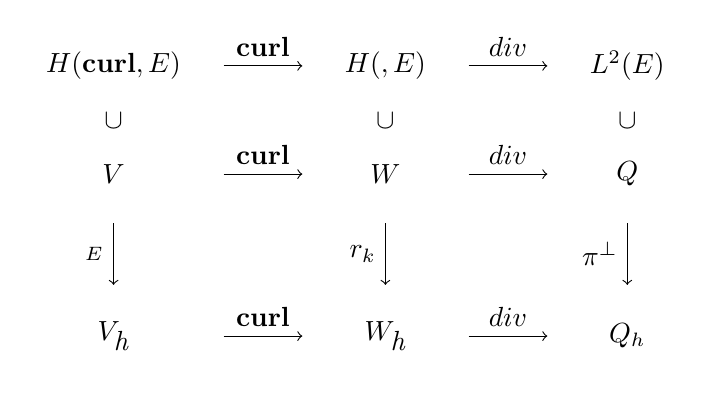
\begin{tikzpicture}[point/.style={circle, inner sep=0pt, minimum size=2pt,fill=red}]
            \matrix[column sep = 1.82mm, row sep = 1.1mm, ampersand replacement = \&] {
             \node {$\text{H}(\textbf{curl},E)$};  
              \& \node (n0) {};
              \& \node      {};
              \& \node (n1) {};
              \& \node (n2) {};
              \& \node {$\text{H}(\Div, E)$}; 
              \& \node (r1c7) {};
              \& \node {};
              \& \node {};
              \& \node (r1c10) {};
              \& \node {$L^2(E)$};\\
             \node (n3) {}; \&\&\&\&\& \node (n5)   {};
              \& \node (r2c7) {};
              \& \node {};
              \& \node {};
              \& \node {};
              \& \node (r2c11) {};\\
             \node (n4) {}; \&\&\&\&\& \node (n6)   {};
              \& \node (r3c7) {};
              \& \node {};
              \& \node {};
              \& \node {};
              \& \node (r3c11) {};\\
             \node (v)  {$V$}; \&\node(fromV){};\&\&\&\node(toW){};\& \node (w) {$W$};
              \& \node (r4c7) {};
              \& \node {};
              \& \node {};
              \& \node (r4c10) {};
              \& \node {$Q$};\\
             \node (n7) {}; \&\&\&\&\& \node (n8)   {};
              \& \node {};
              \& \node {};
              \& \node {};
              \& \node {};
              \& \node (r5c11) {};\\
             \node      {}; \&\&\&\&\& \node        {}; 
              \& \node {};
              \& \node {};
              \& \node {};
              \& \node {};
              \& \node {};\\
             \node      {}; \&\&\&\&\& \node        {}; 
              \& \node {};
              \& \node {};
              \& \node {};
              \& \node {};
              \& \node {};\\
             \node (n11)    {}; \&\&\&\&\& \node (n12) {};
              \& \node {};
              \& \node {};
              \& \node {};
              \& \node {};
              \& \node (r8c11) {};\\
             \node {$V_{\textit{h}} $};                                 
              \& \node (n13) {};
              \& \node       {};
              \& \node (n14) {};
              \& \node (n15) {};
              \& \node {$W_{\textit{h}} $}; 
              \& \node (r9c7) {};
              \& \node {};
              \& \node {};
              \& \node (r9c10) {};
              \& \node {$Q_h$};\\
             };
            \draw[->] (n0) to node[above] {$\textbf{curl}$} (n2); 
            \draw[->] (fromV) to node[above] {$\textbf{curl}$} (toW); 
            \draw[white] (n3) to node {{\color{black}$\cup$}} (n4);
            \draw[white] (n5) to node {{\color{black}$\cup$}} (n6);
            \draw[->] (n7) to node[left] {$\bw_E$} (n11); 
            \draw[->] (n8) to node[left] {$\boldsymbol{r}_k$} (n12); 
            \draw[->] (n13) to node[above] {$\textbf{curl}$} (n15); 
            \draw[->] (r1c7) to node[above] {$\text{div}$} (r1c10);
            \draw[->] (r4c7) to node[above] {$\text{div}$} (r4c10);
            \draw[->] (r9c7) to node[above] {$\text{div}$} (r9c10);
            %\draw[white] (r2c7) to node {{\color{black}$\cup$}} (r3c7);
            \draw[white] (r2c11) to node {{\color{black}$\cup$}} (r3c11);
            \draw[->] (r5c11) to node[left] {$\pi^{\perp}$} (r8c11);
        \end{tikzpicture}
    \end{center}
\begin{equation}\label{push-forward}
  \mbox{\color{red} \ldots \mbox{push-forward} de los interpoladores\\
    y que los pull--backs conmutan con los interpoladores}
\end{equation}
{\bf hcurl}
  
\begin{lemma} \label{aux_label7}
Let $\hat E$ be the reference prism~(\ref{defi_of_ref_prism}) and
let $P_{\hat E}$ be the space in~(\ref{spaceFEprismHcurl}), that is,
\begin{IEEEeqnarray*}{rCl}
  P_{\hat{E}} & = & R_k(\hat{x}_1,\hat{x}_2) \otimes P_k(\hat{x}_3) \times 
            P_k(\hat{x}_1,\hat{x}_2) \otimes P_{k-1}(\hat{x}_3).
\end{IEEEeqnarray*}
Provided the matrix $M_E$ is block--diagonal in this manner
\begin{IEEEeqnarray*}{rCl}
  M_E & = & \blockdiag{m_{1,1}}{m_{1,2}}{m_{2,1}}{m_{2,2}}{m_{3,3}}\mbox{,}
\end{IEEEeqnarray*}
then $P_{\hat{E}}$ is invariant by transformation~(\ref{transfHcurl}).
\end{lemma}
\begin{proof}
  Starting with transformation~(\ref{transfHcurl}) take 
  $\hat{\bu}=(\hat u_1,\hat u_2,\hat u_3)'\in P_{\hat E}$
  and $\bu := (M_E^{-t}\hat{\bu})\circ F_E^{-1}$.
  Let 
  \[
    M_2 = \left(
    \begin{array}{cc}
      m_{1,1}  & m_{1,2}\\
      m_{2,1}  & m_{2,2} 
    \end{array}
    \right)
  \]
  and let $m_{i,j}^{(-1)}$ denote the coefficients of the inverse.
  By definition, 
  $(\hat u_1,\hat u_2)' = \hat{q}(\hat\bp + \hat{\boldsymbol{s}})$ for some
  $\hat\bp$, $\hat{\boldsymbol{s}}$ as in~(\ref{defSk}) and~(\ref{defRk}) and
  $\hat{q}\in P_{k}(\hat x_3).$ Using the blocks of $M_E$ and the tensor nature of
  $P_{\hat E}$,
  \begin{IEEEeqnarray*}{rCl}
    (\hat u_1(\bx),\hat u_2(\bx))' & = & (\hat{q}M_2^{-t}(\hat\bp + 
      \hat{\boldsymbol{s}}))(M_E^{-1}\bx - M_E^{-1}\bx_E)\\
    & = & \hat{q}(m_{3,3}^{(-1)}(x_3-x_{E,3}))(M_2^{-t}(\hat\bp + 
      \hat{\boldsymbol{s}}))(M_2^{-1}\bx - M_2^{-1}\bx_E).
  \end{IEEEeqnarray*}
  Now, $\hat{q}(m_{3,3}^{(-1)}(x_3-x_{E,3}))$ is a polynomial $q(x_3)$ with the
  same 
  degree as $\hat{q}$ is qith respect to $\hat x_3$. Furthermore,
  as by Remark~(\ref{aux_label6}) $\hat{\boldsymbol{s}}$ has degree $\leqslant k-1$,
  $(M_2^{-t}(\hat\bp + \hat{\boldsymbol{s}}))(M_2^{-1}\bx - M_2^{-1}\bx_E)$
  can be seen as
  $M_2^{-t}(\bp(x_1,x_2) + \hat{\boldsymbol{s}}(M_2^{-1}\bx))$ with $\bp$
  having the expected degrees. And now
  \begin{IEEEeqnarray*}{rCcCl}
    M_2^{-t}\hat{\boldsymbol{s}}(M_2^{-1}\bx)\cdot(x_1,x_2)'
        &=& 
    \hat{\boldsymbol{s}}(M_2^{-1}(x_1,x_2)')\cdot M_2^{-1}(x_1,x_2)' &=& 0.
  \end{IEEEeqnarray*}
  The invariance of the third component of elements in $P_{\hat E}$ is
  an immediate consequence of the affine nature of the coordinate change.
\end{proof}
%=======================================================================
%\begin{remark} this is not a restriccion...
%  \begin{figure}
%    \centering
%    *** ***
%    \caption{hybrid mesh}\label{obliquePrism}
%  \end{figure}
%  dibujo prisma oblicuo subdividido: tetra + prism + pyramid. Figure~\ref{obliquePrism}
%\end{remark}
%=======================================================================
\begin{lemma} Let a physical prism $E = F_E(\hat{E})$ for $F_E$ as in~(\ref{aux_label8}).
Given $\hat\bu$ defined in $\hat{E}$ let $\bu$ in $E$ dtermined by~(\ref{transfHcurl}), and
let $\hat\btau$, $\btau$, $\hat\bnu$ and $\bnu$ be tangents and normals in
$\hat E$ and $E$ related by~(\ref{aux_label10}) and~(\ref{aux_label9}). Suppose
we define degrees of freedom of $\bu$ on $E$ as
\begin{IEEEeqnarray}{ll}
    \label{momentos1hcurlPhys}  
    \varphi_{\be_i,p}\,(\bu) = 
    \int_{\be} \bu \cdot \boldsymbol{\tau} \,q\, ds  
        & q\in P_{k-1}\mbox{,} \\
    \IEEEeqnarraymulticol{2}{l}{\nonumber\mbox{ for each edge $\be$ with unit tangent } \boldsymbol{\tau} \mbox{;}}\\[8pt]
    \label{momentos2hcurlPhys} 
    \varphi_{f,\bq}\,(\bu) =  
    \int_{f} \bu \cdot \bq_0\,
    dS\mbox{, } &\bq_0 = (\det M_E\|M_E^{-t}\hat\bnu\|)^{-1} M_E\hat{\bq}_T\\
    &\hat{\bq}_T := (\hat\bnu\times\hat\bq)\times\hat\bnu\\
    &\mbox{$\hat\bq$ as in~(\ref{momentos2hcurl})--(\ref{momentos5hcurl})}.\\[8pt]
    \label{momentos6hcurlPhys}
    \varphi_{\br}(\bu) = 
    \int_{E} \bu \cdot \br \, d\bx\mbox{, }&\br = (\det M_E)^{-1} M_E\hat\br \circ F_E^{-1}\\
    &{\nonumber\hat\br \in P_{k-2,k-2} \times P_{k-3,k-1}.}
\end{IEEEeqnarray}
Provided $\det > 0$, the degrees of freedom are identical
\end{lemma}
\begin{proof}
  Edge dofs: ver foto
  Take a param $\hat{\boldsymbol{\alpha}}(t):I=[0,1]\to \hat\be$ such that
  $\hat\btau=\stackrel{.}{\hat{\boldsymbol{\alpha}}}(t)/\|\stackrel{.}{\hat{\boldsymbol{\alpha}}}(t)\|$.
  As  a jacobian maps tangents into tangents,
  $\boldsymbol{\alpha}(t)=M_E{\hat\bx}(t) + \bx_E$ parameterizes
  $\be$. Then\\
  Edge dofs:
  \begin{IEEEeqnarray*}{rCl}
    \int_{\be}(q\bu)\cdot d\boldsymbol{\alpha}
    &=&\int_{I}
    q\bu(F\hat\bx(t)))\cdot M_E
    \stackrel{.}{\hat{\boldsymbol{\bx}}}(t)dt  \\[5pt]
    &=&\int_{I}
    \hat q(\hat\bx(t)) M_E^{-t}
    \hat\bu(\hat\bx(t))\cdot M_E\stackrel{.}{\hat{\boldsymbol{\bx}}}(t)dt\\[5pt]
    &=&\int_{\hat\be}(\hat q\hat\bu)\cdot d\boldsymbol{\hat\alpha}.
  \end{IEEEeqnarray*}
  Face dofs: 
  \begin{IEEEeqnarray*}{rCl}
    \int_{\hat f} \hat\bv\times\hat\bnu\cdot\hat\bq\times\hat\bnu\,d\hat S 
    & = & \int_{\hat f} (\hat\bnu\times\hat\bq)\times\hat\bnu\cdot\hat\bu\,d\hat S \\
    & = & \int_{\hat f} \det M_E\|M_E^{-t}\hat\bnu\| \bq_0 (F\hat\bx) \cdot \bu(F\hat \bx) d\hat S \\
    & = & \int_{ f} \bq_0 (\bx) \cdot \bu( \bx) d S
  \end{IEEEeqnarray*}
  Vol dofs:
  \begin{IEEEeqnarray}{rCl}
    \int_{E}\bv\cdot\br\,d\bx
    & = & 
    \int_{\hat E}M_E^{-t}\hat\bv(F_E^{-1}\bx)\cdot
      (\det M_E)^{-1}M_E\hat\br(F_E^{-1}\bx)\,d\hat\bx.\\
    & = & 
    \int_{\hat E}\hat\bv(\hat\bx)\cdot\hat\br(\hat\bx)\,d\hat\bx.
  \end{IEEEeqnarray} 
\end{proof}

\begin{lemma} The finite element in Definition~\ref{edgeelement}  is conforming
in $H\curl$ and unisolvent.
  theorem 8 page 75 in~\cite{nedelec2} is incomplete, because it is only on
  the reference element.
\end{lemma}

\begin{lemma} >Provided $\det M^{t} > 0$?, the edge element interpolators satisfy
\begin{IEEEeqnarray}{rCl}\label{piTransformado}
    \wku(\hat{\bx}) & = & M^{t} \bw_E\bu(F_E(\hat{\bx}))
\end{IEEEeqnarray}
That is, the interpolator commutes with the coordinate change~(\ref{transfHcurl}).
\end{lemma}
\begin{proof} 
\end{proof}

{\bf hcurl end}

{\bf hdiv begin}

\begin{lemma}\label{aux_label13} Let $\hat E$ be the reference prism~(\ref{defi_of_ref_prism}) and
let $P_{\hat E}$ be the space in~(\ref{prismaticSpace}).
Provided the matrix $M_E$ is block--diagonal as in Lemma~\ref{aux_label7},
then $P_{\hat{E}}$ is invariant by transformation~(\ref{transfDiv}).
\end{lemma}
\begin{proof} The proof uses the same straightforward approach as the proof of 
Lemma~\ref{aux_label7} and in a much simpler case. \noindent{\color{BrickRed}pensar esto}   
\end{proof}

\begin{lemma} \label{aux_label12}
The degrees of freedom are identical, surface and volumen integrals:
in which the faces are related by $F\hat{f} = f$.
\begin{IEEEeqnarray}{cCccl}
    \label{momentos1hdivPhys} 
    \rho_{ f,q}(\bv) & = & \int_{f} (\bv\cdot\bnu)q\,dS 
        &\quad & \mbox{for } q = \hat{q}\circ F_E^-1, \hat{q} \in P_{k-1}(\hat{f})\mbox{,}\\
    \nonumber&&&\quad&\mbox{if $ \hat{f} =  \hat{f}_3$ or $ \hat{f}_4$;}\\[5pt]
    \label{momentos2hdivPhys}
    \rho_{ f,q}(\bv) & = & \int_{f} (\bv\cdot\bnu)q\,dS 
        &\quad & \mbox{for } q = \hat{q}\circ F_E^-1, \hat{q} \in Q_{k-1, k-1}(\hat f)\mbox{,}\\
    \nonumber&&&\quad&\mbox{ if $ \hat{f} =  \hat{f}_1$, $ \hat{f}_2$ or $ \hat{f}_5$;}\\[5pt]
    \label{momentos3hdivPhys}
    \rho_{ \br}(\bv) & = & \int_{{E}} \bv\cdot\br\,d\bx 
        &\quad& \mbox{for }\br = M_E^{-t}\hat\br\circ F_E^{-1}, \hat\br\in (P_{k-2,k-1})^2 \times P_{k-1,k-2};
\end{IEEEeqnarray}
\end{lemma}
\begin{proof}
  Face dofs, by~(\ref{transfDiv}) and~(\ref{surface_diffs})
  Vol dofs
  \begin{IEEEeqnarray}{rCcCl}
    \int_{E}\bv\cdot\br\,d\bx
    & = & 
    \int_{\hat E}M_E\hat\bv\cdot M_E^{-t}\hat\br\,d\hat\bx.
    & = & 
    \int_{\hat E}\hat\bv\cdot\hat\br\,d\hat\bx.
  \end{IEEEeqnarray}
\end{proof}

\begin{lemma}
  If $\bu\in P_{E}$ is such that all the
  dofs~(\ref{momentos1hdivPhys}) or~(\ref{momentos2hdivPhys}) vanish
  on the respective face $f$, then the normal component of $\bu$ 
  vanishes identically on $f$.
\end{lemma}
\begin{proof}
  This fact is stated in the proof of Theorem 4, page $66$ of~\cite{nedelec2} 
  only for the reference prism. By transforming the degrees of freedom to 
  the faces of $\hat E$ and back to the faces of $E$ using Lemma~\ref{aux_label12}
  we get the result.
\end{proof}
\begin{lemma}
  If $\bu\in P_{E}$ is such that all the
  dofs~(\ref{momentos1hdivPhys})--(\ref{momentos3hdivPhys}) vanish, 
  then $\bu$ vanishes identically on $E$.
\end{lemma}
\begin{proof}
  In the case of the reference prism $\hat E$, we refer to the proof of 
  Theorem 4 in page $66$ of~\cite{nedelec2}.
  by the invariance of the finite element space under
  the change~(\ref{transfDiv}) (Lemma~\ref{aux_label13}) we have our result.
\end{proof}
\begin{corollary}
  Finite Element on $E$ is $H(\dv)$--conforming and unisolvent.
\end{corollary}
\begin{corollary}
  For any $\bv\in W^{1,1}(E)$ expressions 
  ~(\ref{momentos1hdivPhys})--(\ref{momentos3hdivPhys}) 
  determine a well defined local interpolate
  $\br_E\,\bu$ defined as the unique finite element function in $P_E$ such that
  \begin{IEEEeqnarray}{lClc}
    \rho_{f,\bq}\,(\bv - \br_E\,\bu) & = & 0 &
    \quad\mbox{for $\rho_{f,\bq}$ as in~(\ref{momentos1hdivPhys})
      and~(\ref{momentos2hdivPhys})}\\
    \rho_{\br}\,(\bv - \br_E\,\bu) & = & 0 &
    \quad\mbox{for $\rho_{\br}$ as in~(\ref{momentos3hdivPhys})}.
  \end{IEEEeqnarray}
\end{corollary}
And the momentos3hdivPhyswt important
\begin{corollary}
  Given $\bu \in W^{1,1}(E)$, then
  \begin{IEEEeqnarray}{rCl} \label{div_interp_commutes}
    \rku & = & \det M_E\,(M_E^{-1}\,\br_E\,\bu)\circ F_E\mbox{,}
  \end{IEEEeqnarray}
  that is, the $H(\dv)$ interpolator commutes with the coordinate
  change~(\ref{transfDiv}).
\end{corollary}

{\bf hdiv end}


\begin{remark}
  Unisolvence and conformity of the finite elements on tetrahedra in
  Section~\ref{sec:tetrahedralFEs}
  is proved in~\cite{monk}, Sections 5.4 and 5.5.
\end{remark}
%===========================
% See Lemmas 5.32 and 5.34 in pages 130 and 131 of~\cite{monk}, where
% it is proved for tetrahedra. Exacly the same considerations about the degrees
% of freedom therein apply to prove the Lemma for prisms or pyramids.  
% Ver (3.79) (3.80) en monk: transf. de normales y tangentes.\\\\
%===========================